\section{Deep Reinforcement Q-Learning}

In this first part, we present the work done during the first half of the internship, which consists of a literature review and implementations of deep Q-learning algorithms. The first section exposes the background for the reinforcement learning paradigm, the theoretical foundations for Q-learning and the tabular algorithm. The second section provides a description of deep Q-learning (DQN) and the four DQN algorithms implemented; vanilla, double, dueling and prioritized experience replay. The third section presents frameworQ, a python framework for applying DQN algorithms in customized environments, designed as a DQN baseline for the internship project developed in the second half of the internship.

\subsection{Q-learning}

In this first section of the first part, we present the background, fundamentals, and theoretical foundations for the reinforcement learning framework and Q-learning algorithms. This presentation is inspired by [1] (Tabor, 2020), and [2] (Sutton, Barto, 2018).

\subsubsection{RL background}

\textbf{Reinforcement learning} \\
Reinforcement learning is an area of machine learning concerned with how a decision making agent learns from experience to perform tasks in an environment. The agent, with no prior knowledge, will take actions for which it will be rewarded or punished, and observes the outcomes of these decisions. Through successive interactions with the system, the agent will develop a strategy that maximizes cumulative reward over time, hence adopting an optimal behavior to solve the given problem. The set of all possible states is the state space, and the set of all possible actions is the action space. The environment comprises of everything outside of the agent that it interacts with, and can be any complex model governed by a set of rules. The agent and environment interact at each step of a discrete time sequence $ \{t + 0, t + 1, t + 2, ..., t + f\} $, that is after each transition between two successive states. A full time sequence, from an initial state $s_{t+0}$ to a terminal state $s_{t+f}$, is an episode, or an epoch, and the learning run consists of many episodes. \\

\begin{figure}[h]
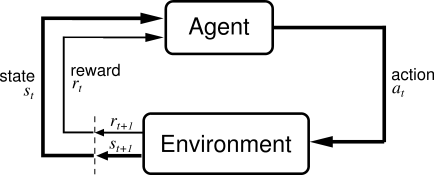
\includegraphics[scale=0.5]{img/I/figtmp7.png}
\centering
\captionsetup{justification=centering}
\caption{RL framework.}
\end{figure}

\textbf{Markov Decision Process} \\
In control theory, the decision making problem an RL agent faces is called an optimal control problem and is formalized as a Markov Decision Process (MDP), a discrete time stochastic control process used to model a decision making process where the controller interacts with a dynamic environment at each discrete timestep $t$ of a sequence. A MDP is defined by the tuple $<S,A,P,R>$, where $S$ is the set of states in the world, $A$ is the set of actions that the agent can take, $P(s_{t+1}|s_t,a_t)$ defines the transition dynamics, and $R(s_t,a_t,s_{t+1})$ is the reward function. A MDP is assumed to satisfy the Markov property, under which the environment's next state $s_{t+1}$ depends only on the current state $s_t$ and the action $a_t$ performed by the agent within this state. The MDP is thus memoryless, meaning that it doesn't rely on the history of past states to perform the next state transition. \\
The sequential decision making process is as follows, at each timestep $t$: 
\begin{enumerate}
    \setlength\itemsep{-0.5em}
    \item the agent makes an observation $x_t$ of  the environment $\varepsilon$ through input signals, i.e. sensors, and approximates the current state $s_t$ of the world with a state-observation pre-processing function $\phi_{s_t} = \phi(x_t) \sim s_t$, in the continuous state space $S$;
    \item the agent performs an action $a_t$ in response to the observed state $s_t$, chosen in the set of possible actions, the discrete action space $A=\{a_1,a_2,...,a_k\}$;
    \item the environment transitions from state $s_t$ to state $s_{t+1}$ as a result of action $a_t$, following the internal dynamics of $\varepsilon$, the finite probability transition matrix $P(s_{t+1}|s_t,a_t)$;
    \item the transition $(s_t,a_t,s_{t+1})$ yields an immediate reward $r_{t+1}$, the instantaneous return of taking action $a_t$ in state $s_t$ according to a reward function $R(s_t,a_t,s_{t+1})$.
\end{enumerate}
The goal of learning in a MDP is to find a policy $\pi(a,s) = p(a|s)$, a mapping from states to actions, that maximizes the long-term benefit, the sum of rewards that follow current time $t$.
As tasks are performed by completing a finite sequence of actions, a discount factor $\gamma \in \ ]0, 1[$ specifies how much immediate rewards are favored over distant rewards within a finite time horizon $T$. Within a finite horizon $T$, the MDP, although possibly arbitrarily large, is guaranteed to be finite. The future discounted reward at time $t$ is:
\[ 
\begin{split}
G_t &= \sum_{k=t}^{t+T} \gamma^{(k-t)} \cdot r_{k+1} = r_{t+1} + \gamma \cdot r_{t+2} + \gamma^2 \cdot r_{t+3} + \gamma^3 \cdot r_{t+4} + ... \\
&= r_{t+1} + \gamma \cdot (r_{t+2} + \gamma \cdot r_{t+3} + \gamma^2 \cdot r_{t+4} + ...) \\
&= r_{t+1} + \gamma \cdot G_{t+1}
\end{split}
\]

\textbf{Optimal action-value Q-function} \\
In environment $\varepsilon$, the transition $(s_t, a_t, s_{t+1}, r_{t+1})$ is not deterministic but stochastic, and the future discounted reward may differ between rollouts due to uncertainty over outcomes. Following the policy $\pi(a,s)$, the value function returns the expected discounted reward for being in the state $s_t$ over all possible trajectories:
\[ V_{\pi}(s) = \mathbf{E}_{\pi}[G_t|s_t=s,\pi] = \mathbf{E}_{\pi}[r_{t+1} + \gamma \cdot G_{t+1}|s_t=s,\pi] \]
With probabilistic state transition dynamics, the expected reward is: 
\[ r(s,a)=\mathbf{E}[r_t|s_{t-1}=s,a_{t-1}=a]=\sum_rr \sum_{s'}p(s',r|s,a) = \sum_{s',r}p(s',r|s,a) \cdot r \]
Thus, the value function becomes:
\[
\begin{split}
V_{\pi}(s) &= \sum_a\pi(a,s)\sum_{s',r}p(s',r|s,a)[r+\gamma \cdot \mathbf{E}_{\pi}[G_{t+1}|s_{t+1}=s']] \\
&= \sum_a\pi(a,s)\sum_{s',r}p(s',r|s,a)[r+\gamma \cdot V_{\pi}(s')]
\end{split}
\]
The recursion derived below is the Bellman equation, a recursive relationship between successive value functions in a MDP. It states that the value of a current state $s_t$ equals the value of the expected next state $s_{t+1}$, discounted by $\gamma$, and incremented by reward $r_{t+1}$.
\\

From the value function and with a fixed action $a_t$ at timestep $t$, the action-value Q-function can be expressed, the value of taking action $a_t$ in state $s_t$ following policy $\pi(a,s)$:
\[
\begin{split}
Q_{\pi}(s,a) &= \mathbf{E}_{\pi}[G_t|s_t=s,a_t=a,\pi] = \mathbf{E}_{\pi}[r_{t+1} + \gamma \cdot G_{t+1}|s_t=s,a_t=a,\pi] \\
&= \mathbf{E}_{\pi}[r_{t+1}+\gamma \cdot V_{\pi}(s_{t+1})|s_t=s,a_t=a,\pi] = \sum_{s',r}p(s',r|s,a)[r+\gamma \cdot V_{\pi}(s')] 
\end{split}
\]
The action-value Q-function assesses the quality of policies based on the value function and enables to rank the expected discounted rewards over states and actions. Thus, by maximizing the action-value Q-function, the agent derives the policy with the greatest expected return, the optimal policy $\pi^*(a,s)$. The  Bellman optimality equation defines the relationship between the optimal value function and the optimal action-value Q-function:
\[ 
\begin{split}
V_\pi^*(s) &= \max_a Q_\pi^*(s,a) \\
&= \max_a \mathbf{E}_{\pi}[r_{t+1}+\gamma \cdot V_{\pi}^*(s_{t+1})|s_t=s,a_t=a,\pi=\pi^*] = \max_a \sum_{s',r}p(s',r|s,a)[r+\gamma \cdot V_{\pi}^*(s')] \\
\end{split}
\]
Consequently, the optimal action-value Q-function is:
\[ Q_\pi^*(s,a) = \mathbf{E}_{\pi}[r_{t+1}+\gamma \cdot \max_{a'} Q_\pi^*(s_{t+1},a')|s_t=s,a_t=a,\pi=\pi^*] = \sum_{s',r}p(s',r|s,a)[r+\gamma \cdot \max_{a'} Q_\pi^*(s',a')] \]

\subsubsection{Q-learning algorithm} \label{basics}

\textbf{Q-learning and value-based RL} \\
Q-learning is a type of reinforcement learning that deals with learning indirectly the optimal policy $\pi^*(s,a)$ from the action-values of state-action pairs, in an unknown environment $\varepsilon$ with stochastic transitions $(s,a,s',r')$, mapping from a continuous state space $S$ to a discrete action space $A$, by optimizing the Q-function $Q_\pi(s,a)$. To do so, it approximates iteratively the optimal Q-function $Q_\pi^*(s,a)$ by selecting the action with the largest expected Q-value $arg\max_{a} Q_\pi(s,a)$ for the current state, learning the expected reward value of the state-action pair. For any finite MDP and given infinite learning time, exploration and exploitation, Q-learning can find an optimal policy: 
\[ \pi^*(s,a) = arg\max_{a}Q_\pi^*(s,a) \]
As the agent learns the optimal policy through the use of (action-) value functions, Q-learning belongs to the broader family of value-based reinforcement learning methods. \\

\textbf{Model-free learning and the explore-exploit trade-off dilemma} \\
Many optimization problems rely on model-based learning, where the complete model of the environment is known and classical dynamic programming techniques allow explicit planning by solving systems of equations. However, in many cases, the inner dynamics of the model is either unknown or too complex, and these methods become unfeasible. \
Contrariwise, Q-learning does not require prior knowledge of the environment, i.e. it is said to be model-free. Here, the probability distribution over transitions $p(s',r|s,a)$ is unknown, and is indirectly estimated by taking actions in a trial and error fashion. Thus, the learning task is completed by alternating between periods of exploration and exploitation. During exploration, the agent takes random actions, which are sub-optimal, in order to discover new states that haven't been visited so far. This allows the learning process to discover new regions of the state space, and avoid getting stuck in a sub-optimal local optimum. In fact, the function to be optimized is generally not convex, and consists of many local optima, which are optimal solutions within a neighboring set of candidate solutions, and the optimal local optimum being the global optimum, the optimal solution among all possible solutions. Exploration is meant to discover the widest range of local neighborhoods to gain a macroscopic knowledge over the shape of the function. Exploitation, on the other hand, optimizes the information acquired during exploration on a microscopic level, by finding the local optima within neighborhoods. Here, the agent is greedy to maximize the reward and takes the best known action, by highest Q-value. Therefore, it is during exploitation that the agent learns a solution to the optimization problem, whose quality is however subjected to the amount of previous exploration. This trade-off between exploration and exploitation is called the explore-exploit dilemma, and finding the adequate balance requires to  estimate the opportunity cost of greed. \\

\textbf{Off-policy learning and the epsilon-greedy policy} \\
While there is no ground rule to tackle the explore-exploit trade-off, Q-learning uses an action-selection policy known as epsilon-greedy, or $\epsilon$-greedy. This strategy is referred as off-policy, as the action-selection policy differs from the learned policy $\pi$ by including an epsilon $\epsilon$ threshold for random action selection. At each timestep, the agent will either explore and take a random action with probability $\epsilon$, or exploit and take the best known action for the given state with probability $1-\epsilon$ following the learned behavior policy $\pi$:
\[ 
\epsilon\text{-greedy policy: } a = 
    \begin{cases}
      arg \max_{a}Q_\pi(s,a) & \text{with probability } 1-\epsilon\\
      \text{rand a} \in A & \text{with probability } \epsilon
    \end{cases}
\]
There are many ways to define $\epsilon$, the most common being linear decay. At the beginning of learning, $\epsilon = 1$ as there is no knowledge of the environment to exploit. Then, as the need for exploitation decreases and exploitation becomes more important, $\epsilon$ is decayed linearly to a lower bound $\epsilon_{min}$ and over a period $\epsilon_{dec}$, following an interpolation function:
\[ 
\text{Linear decay: } \epsilon = 
    \begin{cases}
      t \cdot \frac{(\epsilon_{min}-1)}{\epsilon_{dec}} + 1 & \text{if } t < \epsilon_{dec}\\
      \epsilon_{min} > 0 & \text{else}
    \end{cases}
\]
The exploration probability must never end up null, as a continuous state space can never be fully explored by definition. Indeed, Q-learning converges in the long-term towards the best local optimum discovered, but is not guaranteed to discover the global optimum. \\

\textbf{Temporal difference learning and target update} \\
Q-learning learns the optimal Q-function by temporal difference, an iterative update of the Q-values over the difference between new and old estimates for a state-action pair. The mechanism used in temporal difference for creating new estimates from older samples is known as bootstrapping, and, since performed at each iteration, is said to be online. The temporal difference is the difference between a temporal difference target, an estimate of the Q-value for the next state computed from its expected optimal action-value, and the estimate of the Q-value for the current state. The temporal difference, weighted by a learning rate $\alpha$, is incremented to the current Q-value to update the Q-function:
\[ 
\begin{split}
Q_{\pi,t+1}(s_{t},a_{t})&= \mathbf{E}_{\pi}[r_{t+1}+\gamma \cdot \max_{a'} Q_{\pi,t}(s_{t+1},a')|s_t=s,a_t=a, \pi] \\
&=Q_{\pi,t}(s_{t},a_{t})+\alpha \cdot (r_{t+1}+\gamma \cdot \max_{a}Q_{\pi,t}(s_{t+1},a)-Q_{\pi,t}(s_{t},a_{t})) 
\end{split}
\]

\begin{figure}[h]
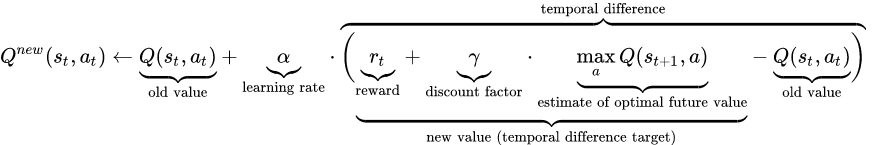
\includegraphics[width=\textwidth]{img/I/Selection_096.png}
\centering
\end{figure}

The learning rate parameter $\alpha$ controls the extent to which new estimates override old ones during the update. It metaphorically represents the speed at which the agent learns. Given infinite iterations of TD, Q-learning converges towards the optimal Q-function:

\[ Q_{\pi,t} \longrightarrow Q_{\pi,t}^*\ \text{, when}\ t \longrightarrow \infty \]

\textbf{Tabular Q-learning algorithm} \\
By the temporal difference definition, the optimization of the Q-function relies on its recursive property, derived from the Bellman optimality equation. A function approximator is therefore necessary to represent the Q-function in a way that is iteratively updateable.
In its original and simplest form, the Q-learning algorithm uses a table as a function approximator to store the Q-values of the Q-function, the Q-table. This Q-table is thus a $(|s|+1)$-dimensional matrix, with entries being the indices for the $|s|$-dimensional states and the $1$-dimensional actions, and the corresponding cells being the Q-values of the state-action pairs. Here, the continuous state space is divided into discrete bins of similar states for a discrete representation in the Q-table. The algorithm is as follows: 
For $E$ episodes, over the sequences from an initial to a terminal state, with total steps $t$, the agent observes the state $s$ and takes the action $a$ according to the $\epsilon$-greedy policy, and the model transitions to the next state $s'$, yielding reward $r'$. From the transition $(s,a,s',r')$, the agent updates, by temporal difference, the Q-value of the state-action pair in the Q-table.

\begin{algorithm}[H]
\small
\caption*{Tabular Q-learning algorithm}
\begin{algorithmic}
    \STATE Initialize step $t = 0$;
    \STATE Initialize $Q$-table $Q$ with $Q(s,a)=0$, $\forall s \in S$, $\forall a \in A$;
    \FOR{episode e = 1,E}
        \bindent
        \STATE Initialize sequence, observe initial state $s_t=\phi(x_t)$;
        \WHILE{$s_t$ not terminal}
            \bindent
            \STATE With probability $\epsilon$ select a random action $a_t \in A$
            \STATE otherwise select action $a_t = arg\max_{a}Q_{\pi,t}(s_t,a)$;
            \STATE Execute $a_t$ in  emulator $\varepsilon$ and observe reward $r_{t+1}$ and next state $s_{t+1}=\phi(x_{t+1})$;
            \STATE Update $Q_{\pi,t+1}(s_{t},a_{t}) =Q_{\pi,t}(s_{t},a_{t})+\alpha \cdot (r_{t+1}+\gamma \cdot \max_{a}Q_{\pi,t}(s_{t+1},a)-Q_{\pi,t}(s_{t},a_{t}))$;
            \STATE Decay $\epsilon$ with linear decay;
            \STATE Increment step $t = t + 1$;
            \eindent
        \ENDWHILE
        \eindent
    \ENDFOR
\end{algorithmic}
\end{algorithm}

\pagebreak